\documentclass[tikz,border=6pt]{standalone}
\usepackage{ctex}
\usepackage{graphicx}
\usepackage{tikz}

\begin{document}
\begin{minipage}{0.98\textwidth}
\centering
\begin{minipage}[t]{0.48\textwidth}
  \centering
  
\includegraphics[width=\textwidth]{real-training-images/training_curves.png}
  
  \small (a) 训练/验证曲线
\end{minipage}
\hfill
\begin{minipage}[t]{0.48\textwidth}
  \centering
  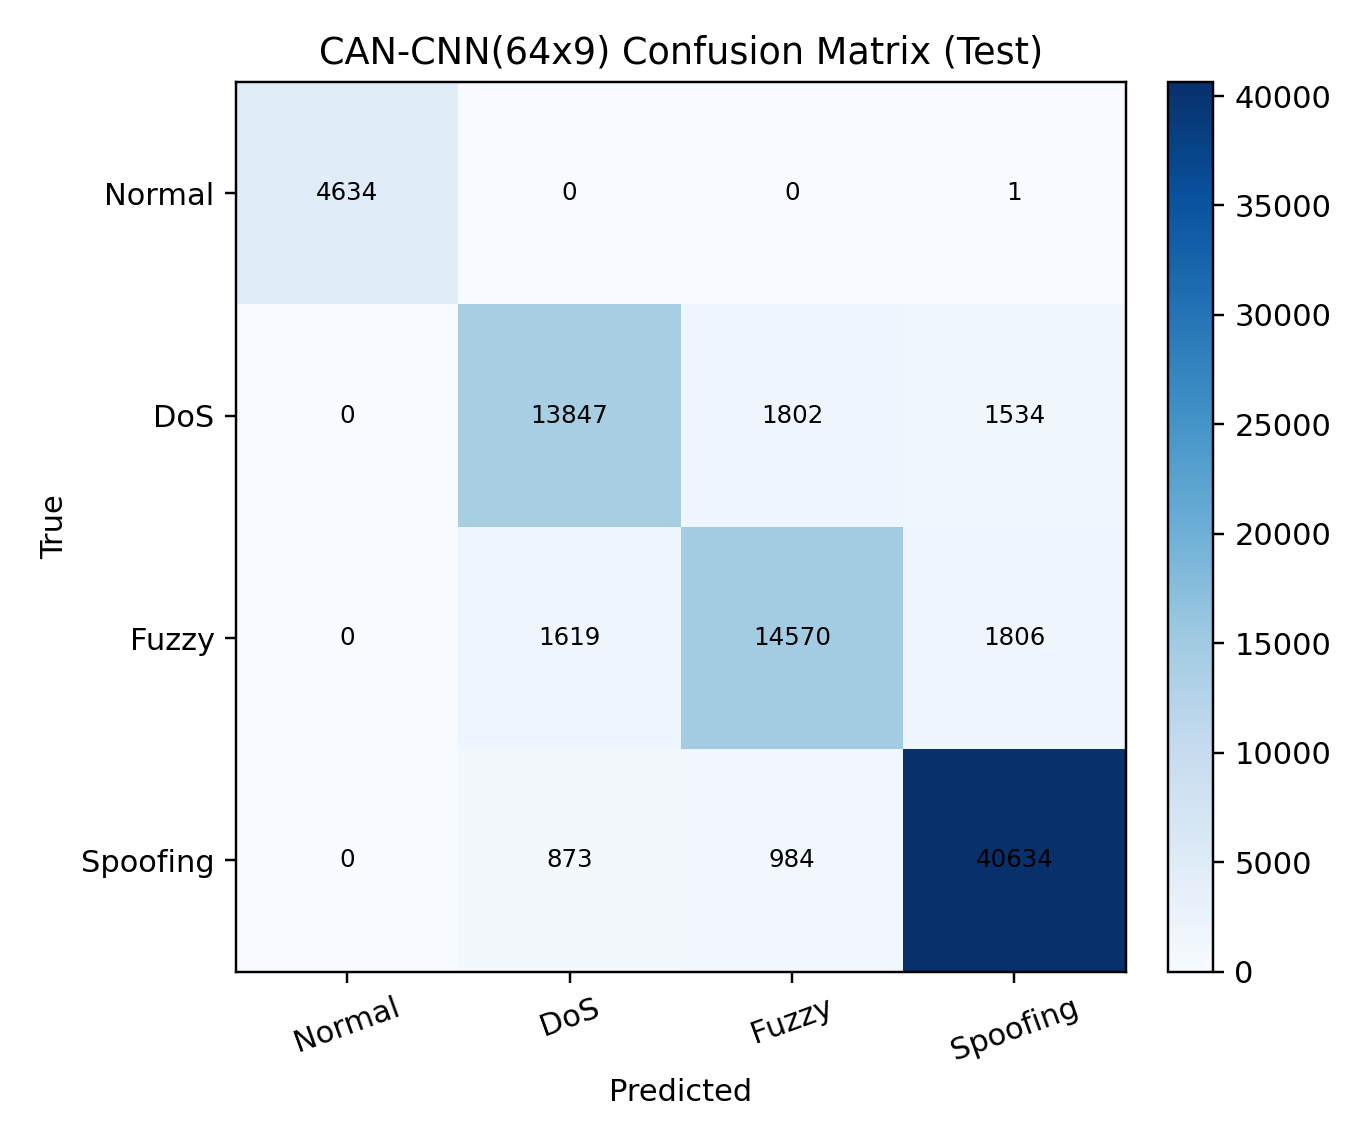
\includegraphics[width=\textwidth]{real-training-images/confusion_matrix_can_cnn64.png}
  
  \small (b) 测试集混淆矩阵
\end{minipage}

\vspace{0.7em}

\begin{minipage}[t]{0.55\textwidth}
  \centering
  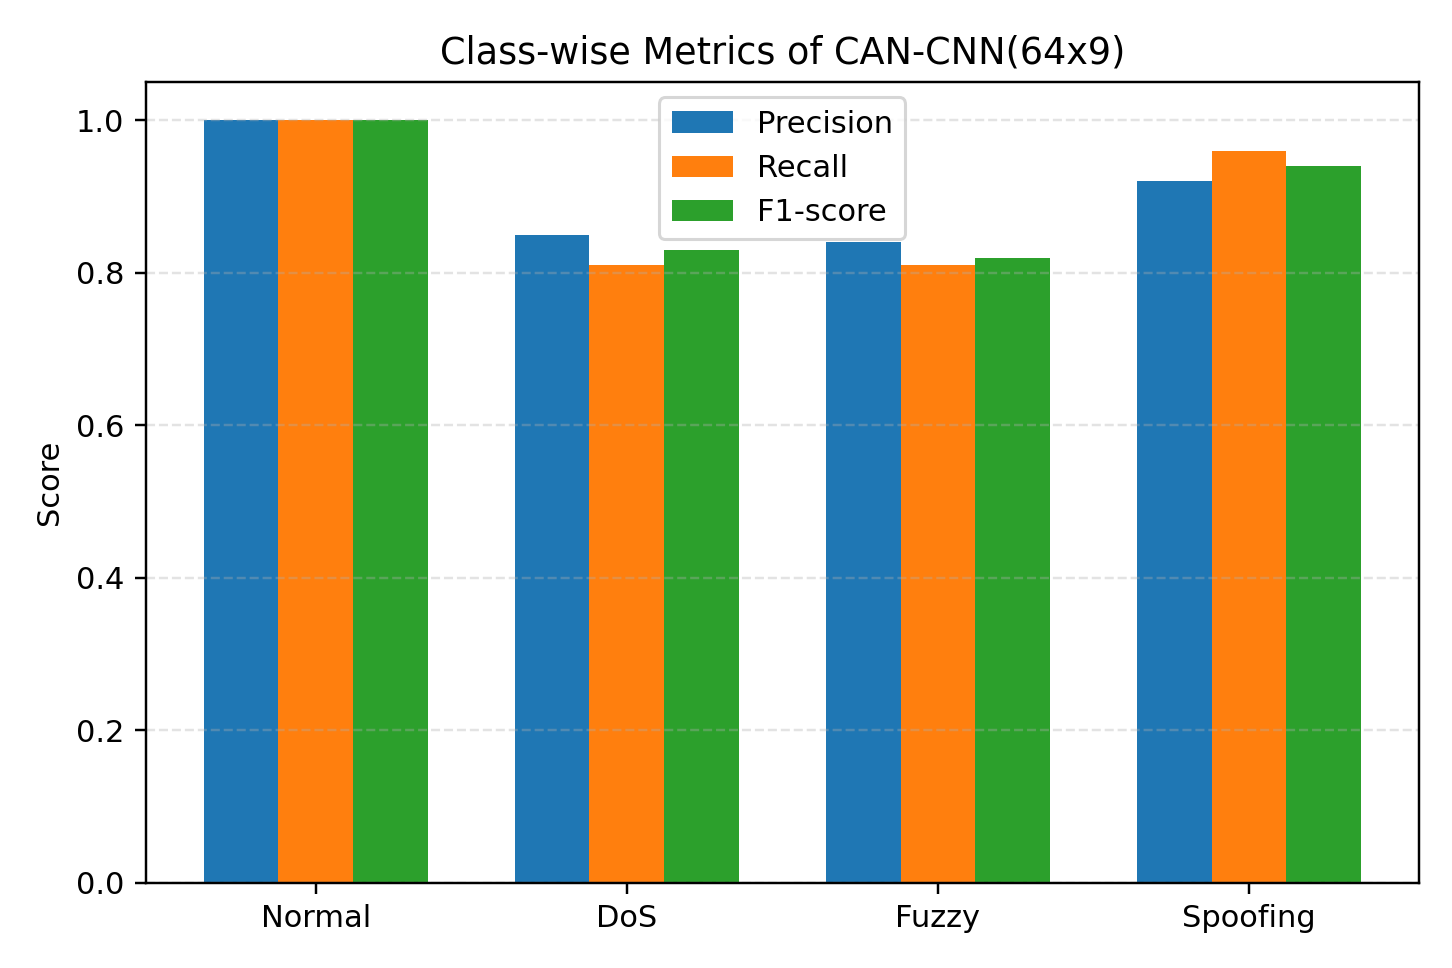
\includegraphics[width=\textwidth]{real-training-images/class_metrics_can_cnn64.png}
  
  \small (c) 各类别 Precision/Recall/F1
\end{minipage}
\hfill
\begin{minipage}[t]{0.40\textwidth}
  \centering
  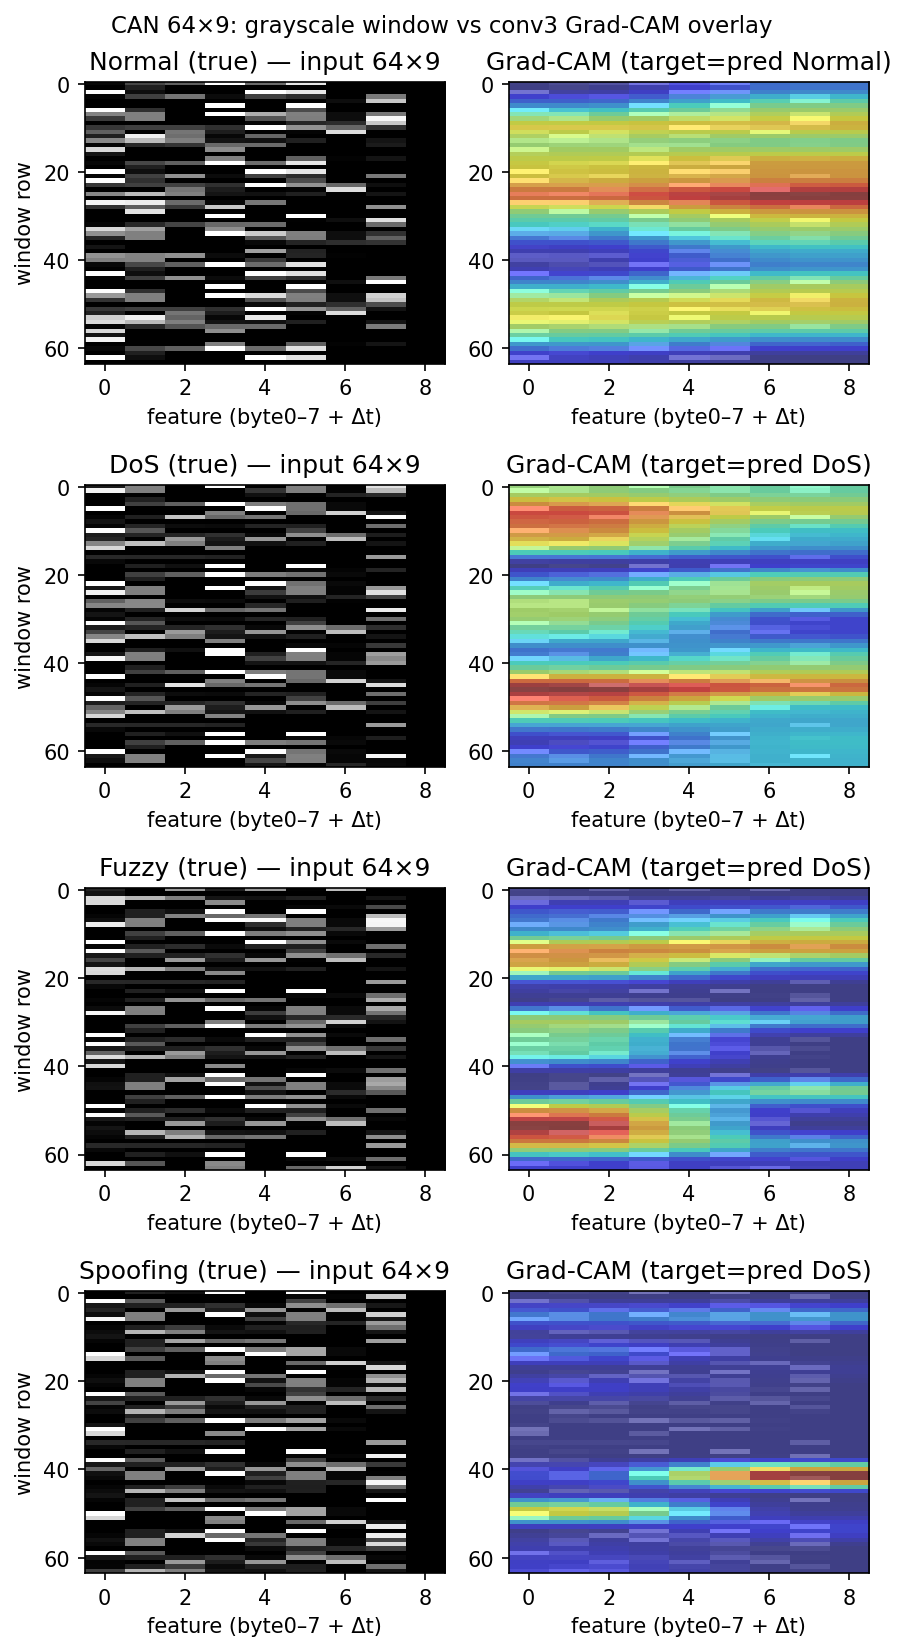
\includegraphics[width=\textwidth]{real-training-images/analysis_result.png}
  
  \small (d) Grad-CAM 可解释性
\end{minipage}

\vspace{0.4em}
\begin{tikzpicture}
  \node[draw=black!35, rounded corners=2mm, fill=blue!7, align=left, inner sep=5pt] {
  全部面板均来自 \texttt{can\_cnn\_64x9} 真实训练与评估结果，集中证明收敛性、可分性与解释性。};
\end{tikzpicture}
\end{minipage}
\end{document}
